\section{Design}\label{sec: Design}
In this section the design and decisions that where made to achieve the laboratory are discussed.

\subsection{Vending machine specification}\label{subsec: Vending machine specification}
Verilog is used to describe a decoder that shall control a seven-segment display with two switches and one button. The given task is as followed:
\\ \\
The design should be implemented on t he PYNQ board using two Pmod 7-segment displays.
VENDMACH is a vending machine that accepts nickels, and dimes, and dispenses gum, apple, or yogurt. A
gum pack costs 10\cent, an apple is 15\cent, and yogurt is 20\cent. The machine is only allowed to accept up to 20\cent. Any
coins inserted that pushes the value beyond 20\cent should be ignored.

\begin{description}
	\item[ - NICKEL]  \t a signal that becomes 1 when a nickel is deposited in the coin slot.
	\item[ - DIME] a signal that becomes 1 when a dime is deposited in the coin slot.
	\item[ - GUM] a signal that becomes 1 when the gum selection button is pressed.
	\item[ - APPLE] a signal that becomes 1 when the apple select ion button is pressed.
	\item[ - YOGURT] a signal that becomes 1 when the yogurt select ion button is pressed.
\end{description}
In addition ion to these “user” inputs, the machine has two control inputs:
\begin{description}
	\item[ - CLOCK] a timing signal that sequences the state transit ions of the machine.
	\item[ - RST] an initialization signal that resets the machine to a suitable starting
	state.
\end{description}
The machine has three outputs:
\begin{description}
	\item[ - MONEY ENTERED] The amount of money inserted into the machine should be displayed on one of the 7-segment Pmod displays. This should update every time a coin is inserted (i.e. 5\cent should read 05). Upon startup or reset, the display should read VEND.
	\item[ - DISPENSED ITEM] The item that was just purchased should be displayed on the 7-segment: g for gum, A for apple, and y for yogurt, as indicated in figure below.
	\item[ - CHANGE] The amount of money returned in change. The machine returns change using only	cents; the number of cents returned should be displayed as a binary number using the on-board LEDs.
\end{description}


\begin{figure}[htbp]
	\centering
	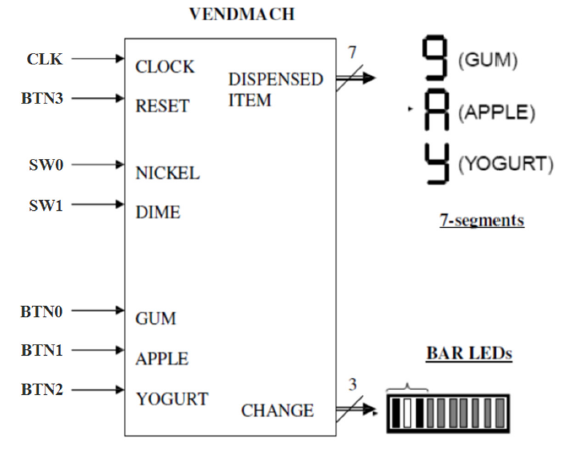
\includegraphics[width=0.7\textwidth]{01_images/Vivado_lab3_DesignSpec3_ModuleOverview.PNG}
	\caption{VENDMACH top level module.}
	\label{fig: Vivado_lab3_DesignSpec3_ModuleOverview}
\end{figure}

The above specification leads to the following table.
\begin{table}[ht]
	\begin{center}
		\begin{tabular}{|| c | c | c | c | c ||} 
			\hline
			  Description & Switches & Displayed Pmod A  \\ [0.5ex] 
			\hline\hline
			Nickel is 5 \cent 	& SW0 	& 	05  	\\ \hline
			Dime is 10 \cent 	& SW1	&	10  	\\ \hline
			
		\end{tabular}
	\end{center}
	\caption{VENDMACH allowed coins.}
\end{table}

\begin{table}[ht]
	\begin{center}
		\begin{tabular}{|| c | c | c | c | c ||} 
			\hline
			Product & Price  & Displayed Pmod B \\ [0.5ex] 
			\hline\hline
			Gum  	& 10 \cent	& g		\\ \hline
			Apple 	& 15 \cent	& A  	\\ \hline
			Yogurt 	& 20 \cent	& y  	\\ \hline
			
		\end{tabular}
	\end{center}
	\caption{VENDMACH products and prices.}
\end{table}

\begin{figure}
	\begin{verbatim}       
	                       000                                  001
       +---------------------+               +---------------------+
       |                     |               |                     |
       | Idle                |<--------------| Reset               |<------+
       | Display OFF         |               | BTN3                |       |
       +---------------------+               +---------------------+-      |
           |                                                               |
           |                                                               |
           |              003                                              |       002
       +---------------------+ Add to coin_val                  +---------------------+
       |                     |---------------+                  | Delay               |
       | Coin entered show   |               |                  | 3s                  |
       | coin_val on Pmod A  |<--------------+                  |                     |
       +---------------------+                                  +---------------------+
           |                                                              / \ 
           |                                                             / | \
           |              004                                              |       007
       +---------------------+                                  +---------------------+
       | IF value > Gum      |                                  | Vend                |
       | & coin_val > 10     |--------------------------------->| Display "VENT"      |
       | Display 'g' by BTN0 |                                  | Disp returned cents |
       +---------------------+                                  +---------------------+
           |                                                              / \ 
           |                                                             / | \
           |              005                                              |
       +---------------------+                                             |
       | IF value > Apple    |                                             |
       | & coin_val > 15     |------------------->------------------->-----+
       | Display 'A' by BTN1 |                                             |
       +---------------------+                                             |
           |                                                               |
           |                                                               |
           |              006                                              |
       +---------------------+                                             |
       | IF value > Yogurt   |                                             |
       | & coin_val > 20     |------------------->------------------->-----+
       | Display 'y' by BTN2 |                                           
       +---------------------+                                           

	\end{verbatim}
	\caption{VNEDMACH state machine.}
\end{figure}
%\begin{figure}[htbp]
%	\centering
%	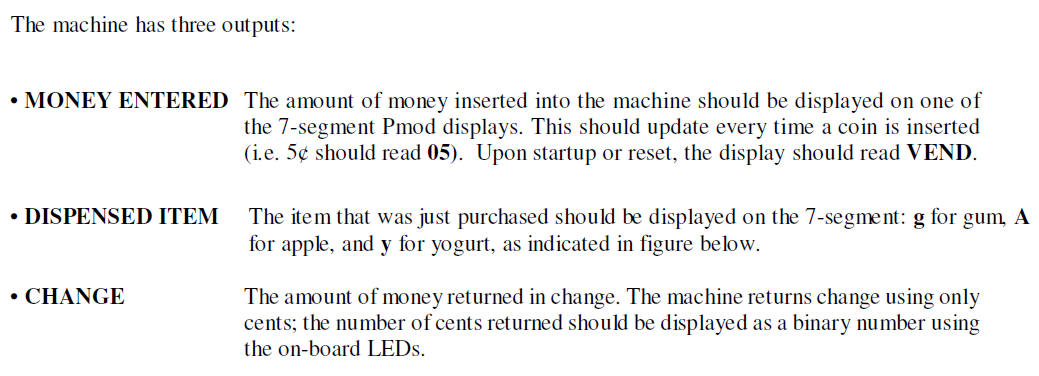
\includegraphics[width=1.0\textwidth]{01_images/Vivado_lab3_DesignSpec2.PNG}
%	\caption{VENDMACH Design Specification}
%	\label{fig: Vivado_lab3_DesignSpec2}
%\end{figure}

As software package to implement the decoder in Verilog Vivado 2017.2 is used. 
%
%\subsection{Part II - Hardware Implementation \& Modular Design}\label{subsec: Hardware Implementation Modular Design}
%For the second part a hierarchical design is achieved including the implementation and generation of a bit stream to use hardware or more specific the PYNQ development board. Therfore the folowing task is given:
%\\
%\\
%In this part, you will modify your code from Part I. Instead of only using one button and one switch, you will
%design your Verilog code to display on four seven-segment displays by pressing the four buttons on the PYNQ
%board. Each seven-segment display will correspond to one button (i.e., BTN0 lights up the right-most seven-segment
%display and BTN1 will light up the adjacent seven-segment display and so on). Make sure that when a
%button is released, the corresponding seven-segment display turns OFF. Only one seven-segment display should
%be on at any given time.
%\\
%\\
%To realize the constrained file the PYNQ reference manual was used to allocate the right pins for the switches and buttons, figure \ref{fig: PYNQ_BasicIO} shows the basic I/O pins assignment of the PYNQ development board.
%\begin{figure}[H]
%	\centering
%	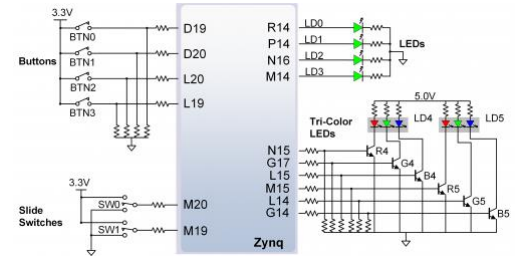
\includegraphics[width=0.6\textwidth]{01_images/PYNQ_BasicIO.png}
%	\caption{Schematic PYNQ Basic I/O. \cite{PYNG_RM}}
%	\label{fig: PYNQ_BasicIO}
%\end{figure}
%The one of solution to part II is two concatenated case statements. The first case is used to check for the button press and the second to switch the seven-segment display to show the number as defined by the two switches SW0 and SW1. The used code is listed in the following three listening \ref{lst: decoder part II}, \ref{lst: decoder top level part II}, and \ref{lst: decoder Constrains part II}.
%
%\subsection{Part III - Laboratory Exercise}\label{subsec: Part III - Laboratory Exercise}
%The third part of the lab combines part one and part two to a final design that uses a modified decoder version of part two and a clock divider to print out the words, PYNQ, FPGA, IS, and COOL with the seven-segment display. The clock divider is used to slow down the 125 MHz clock to 125 Hz, the relation ship of clock divider an decoder is shown in figure \ref{fig: Vivado_lab2_part3_block_diagram}. Switches SW0 and SW1 defines which word will be shown on the displays if the button BTN0 is pressed, as shown in figure \ref{fig: Vivado_lab2_part3_InAndOutTable}. The task is described as followed in the lab report: \\   
%\\
%In this part, you will create a time multiplexed seven-segment decoder using the block diagram shown in Figure
%8 as a guide. You will need to create a multiplexer in order to display more than one seven-segment
%simultaneously. Design the multiplexer to enable each digit for 8ms, or a 125Hz refresh rate. Remember, these
%Pmods have a shared digit select pin. Most multi-digit displays would have a separate digit select pin for each
%digit. Table 3 shows the required outputs for the required input combinations.
%
%\begin{figure}[H]
%	\centering
%	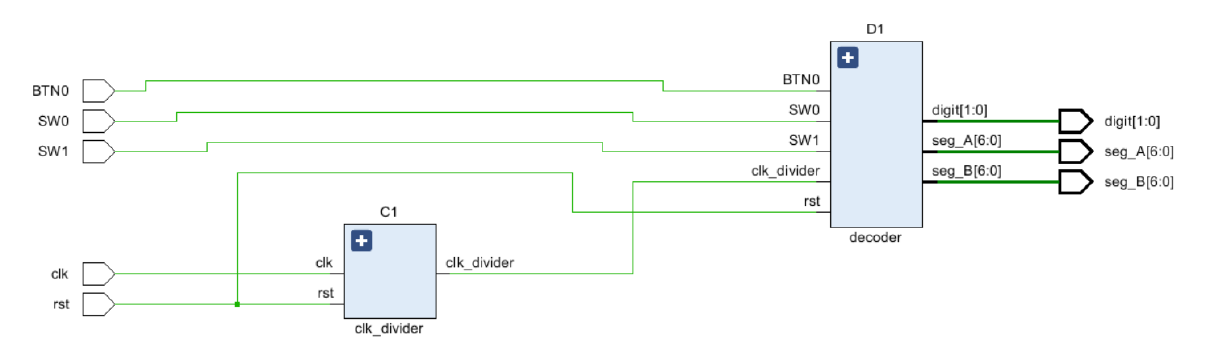
\includegraphics[width=1.0\textwidth]{01_images/Vivado_lab2_part3_block_diagram.PNG}
%	\caption{Part III block diagram. \cite{PYNG_RM}}
%	\label{fig: Vivado_lab2_part3_block_diagram}
%\end{figure}
%\begin{figure}[H]
%	\centering
%	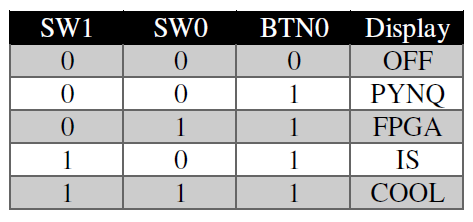
\includegraphics[width=0.5\textwidth]{01_images/Vivado_lab2_part3_InAndOutTable.PNG}
%	\caption{Part III inputs and outputs. \cite{PYNG_RM}}
%	\label{fig: Vivado_lab2_part3_InAndOutTable}
%\end{figure}
%
%The clock divider is realized with a counter that counts up until the divider ratio is reached of 500,000 as calculated with equation \ref{eq: div ratio}.
%
%\begin{equation} \label{eq: div ratio}
%	Divider\ ratio = \frac{f_1}{f_2 * 2} = \frac{125 MHz}{125 Hz * 2} = 500,000
%\end{equation}
%Therefore, a clk\_temp register is used to count up until the counter value equal or great than 500,000 is reached. In the top module the divided clk\_out of the clk\_divider is wired into the decoder. The reason is why the clock needs to be divided at the first placed is that a two fast clock would prevent the viability of the seven-segment displays. 
%The decoder is time multiplexed because each seven-segment display has a common carriage line to display ever a number on display A or display B. Therefor, a time multiplexer was written which is clock depended that each display one after another.
%The time multiplexer is realized with a case statement and a two bit value that iterates trough and each case displays one character of a word. 
%\\ 
%\\
Further improvements that would increase the code quality and re-usability of the  modules would be to change the clk\_divider module that the divider ratio is given as input to the clock divider. 
